\chapter{Archived in February 22, 2024}

The filtering and synchronization process of raw signals was updated to make it easier to use and reduce unnecessary complexities. For reference, below is a copy of derived data was being handled up to the date of this archiving.
\section{Derived Data Description}

The signals generated by this step are located in the following tables:

\begin{itemize}
	\item eeg\_sync
	\item fnirs\_sync
	\item ekg\_sync
	\item gsr\_sync
\end{itemize}

The column \emph{frequency} indicates the frequency of the shared clock which is 200Hz by default. If we include other frequencies in the feature, the value in this column can be used to select the desired one.


\subsection{Derived Data Files}

The following folders contain several versions of derived data at various synchronization frequencies:
\begin{itemize}
  \item \texttt{fnirs\_10hz} contains synchronized fNIRS signals and task data at 10 Hz sampling rate.
  \item \texttt{fnirs\_500hz} contains synchronized fNIRS signals and task data at 500 Hz sampling rate.
  \item \texttt{eeg\_500hz} contains synchronized EEG signals and task data at 500 Hz sampling rate.
  \item \texttt{ekg\_500hz} contains synchronized EKG signals and task data at 500 Hz sampling rate.
  \item \texttt{gsr\_500hz} contains synchronized GSR signals and task data at 500 Hz sampling rate.
  \item \texttt{fnirs\_eeg\_ekg\_gsr\_120hz} contains synchronized fNIRS, EEG, EKG, and GSR signals and task data at 120 Hz sampling rate.
  \item \texttt{fnirs\_eeg\_ekg\_gsr\_1200hz} contains synchronized fNIRS, EEG, EKG, and GSR signals and task data at 1200 Hz sampling rate.
\end{itemize}

Each derived data folder contains synchronized fNIRS, EEG, EKG, and/or GSR signals for each task and for the entire experiment for each experiment:
\begin{verbatim}
exp_*/
    all.csv
    rest_state.csv
    finger_tapping.csv
    affective_individual_lion.csv
    affective_individual_tiger.csv
    affective_individual_leopard.csv
    affective_team.csv
    ping_pong_competitive_lion_tiger.csv
    ping_pong_competitive_leopard_cheetah.csv
    ping_pong_cooperative.csv
    minecraft_saturn_a.csv
    minecraft_saturn_b.csv
\end{verbatim}

Each experiment contains the following CSV files, with columns described in \ref{sec:derived_data_cols_desc}:
%
\begin{itemize}
  \item \texttt{all.csv} contains the synchronized signal of all participants for the entire recording sessions, including signals and data in all tasks.
  \item \texttt{rest\_state.csv} contains the synchronized signal and rest state task data.
  \item \texttt{finger\_tapping.csv} contains the synchronized signal and finger tapping task data.
  \item \texttt{affective\_individual\_lion.csv} contains the synchronized signal and individual affective task data for participant using the Lion computer in the lab.
  \item \texttt{affective\_individual\_tiger.csv} contains the synchronized signal and individual affective task data for participant using the Leopard computer in the lab.
  \item \texttt{affective\_individual\_leopard.csv} contains the synchronized signal and individual affective task data for participant using the Leopard computer in the lab.
  \item \texttt{affective\_team.csv} contains the synchronized signal and team affective task data.
  \item \texttt{ping\_pong\_competitive\_lion\_tiger.csv} contains the synchronized signal and ping pong competitive task data between participants sitting on Lion and Tiger stations.
  \item \texttt{ping\_pong\_competitive\_leopard\_cheetah.csv} contains the synchronized signal and ping pong competitive task data between a participant sitting on Leopard station and an experimenter sitting on the Cheetah station.
  \item \texttt{ping\_pong\_cooperative.csv} contains the synchronized signal and ping pong cooperative task data between three participants against an artificial intelligent agent.
  \item \texttt{minecraft\_hands\_on\_training.csv} contains the synchronized signal and Minecraft search-and-rescue hands-on training mission data.
  \item \texttt{minecraft\_saturn\_a.csv} contains the synchronized signal and Minecraft search-and-rescue Saturn A mission data.
  \item \texttt{minecraft\_saturn\_b.csv} contains the synchronized signal and Minecraft search-and-rescue Saturn B mission data.
\end{itemize}

Not all experiments may include the aforementioned CSV files, due to a couple
of primary reasons. Firstly, time constraints can result in certain tasks
remaining incomplete in some experiments. Secondly, instances where the
experiment involves only two participants or the recorded signals are
compromised during certain tasks can also lead to the absence of these CSV
files.

\subsection{Derived Data Columns Descriptions}
\label{sec:derived_data_cols_desc}

The columns in each aforementioned CSV file (e.g., \texttt{rest\_state.csv},
\texttt{ping\_pong\_cooperative.csv}) are detailed in
\autoref{tab:shared_columns}, \autoref{tab:rest_task_columns},
\autoref{tab:finger_task_columns},
\autoref{tab:individual_affective_task_columns},
\autoref{tab:team_affective_task_columns},
\autoref{tab:ping_pong_competitive_task_columns},
\autoref{tab:ping_pong_cooperative_task_columns},
\autoref{tab:minecraft_task_columns}, \autoref{tab:EEG_signals},
\autoref{tab:fNIRS_raw_signals}, and \autoref{tab:fNIRS_signals}.

%---

\begin{table}
    \footnotesize
    \centering
    \begin{tabularx}{\textwidth}{lX}
        \toprule
        Time columns & Description \\
        \midrule
        \texttt{timestamp\_unix} & Unix time (in seconds, with 0.1 microsecond resolution) of when the signals and the task data were recorded and synchronized.\\
        \bottomrule
    \end{tabularx}
    \caption{Columns of time that are common in all CSV files of derived data.}
    \label{tab:shared_columns}
\end{table}

%---

\begin{table}
\centering
\begin{tabularx}{\textwidth}{lX}
    \toprule
Channel & Description \\
\midrule
\texttt{event\_type} & Event labels for the rest state task. Event types include \texttt{start\_task} signifying the start of the task, and \texttt{end\_task} signifying the end of rest state task.\\
\bottomrule
\end{tabularx}
\caption{Rest State Task columns information in the CSV file \texttt{rest\_state.csv} of the derived data.}
\label{tab:rest_task_columns}
\end{table}

%---

\begin{table}
\centering
\begin{tabularx}{\textwidth}{lX}
    \toprule
Channel & Description \\
\midrule
\texttt{event\_type} & Event labels for the finger tapping task. Event types include \texttt{start\_fingertapping\_task} signifying the start of the task and the practice period, \texttt{individual} for the period during which the participants must tap in rhythm by themselves, and \texttt{team} for the period during which the participants must tap in synchronized rhythm with other participants.\\
\texttt{countdown\_timer} & This is the timer displayed to the participants on the monitor signifying the remaining duration of the task's phase.\\
\texttt{lion\_spacebar\_pressed} & \texttt{0} for when the participant on the Lion computer is not pressing and holding down on the spacebar, and \texttt{1} for when the participant is pressing and holding down the space bar.\\
\texttt{tiger\_spacebar\_pressed} & \texttt{0} for when the participant on the Tiger computer is not pressing and holding down on the spacebar, and \texttt{1} for when the participant is pressing and holding down the space bar.\\
\texttt{leopard\_spacebar\_pressed} & \texttt{0} for when the participant on the Leopard computer is not pressing and holding down on the spacebar, and \texttt{1} for when the participant is pressing and holding down the space bar.\\
\bottomrule
\end{tabularx}
\caption{Finger Tapping Task columns information in the CSV file \texttt{finger\_tapping.csv} of the derived data.}
\label{tab:finger_task_columns}
\end{table}

%---

\begin{table}
\centering
\begin{tabularx}{\textwidth}{lX}
    \toprule
    Channel & Description \\\midrule
    \texttt{event\_type} & Event labels for the individual affective task. Event types include \texttt{start\_affective\_task} signifying the start of the task, \texttt{intermediate\_selection} signifying when a participant selects an arousal rating or a valence rating after observing an image, and \texttt{final\_submission} signifying when a participant submits the arousal and valence score for an image. For experiments recorded in April, 2023 onward, there are additional events, including \texttt{show\_blank\_screen} for when a participant's monitor began rendering the blank, black screen, \texttt{show\_cross\_screen} for when the monitor began rendering the black background with a plus symbol in the middle of the screen to center the participant's attention, \texttt{show\_image} for when the monitor began rendering an image at the center of the screen in front of a black background, and \texttt{show\_rating\_screen} for when the monitor began rendering the arousal and valence rating screen at the center of the screen.\\
    \texttt{image\_path} & The image file that was rendered on the participants' monitors.\\
    \texttt{arousal\_score} & The arousal score selected by the participant during the \texttt{intermediate\_selection} and \texttt{final\_submission} events.\\
    \texttt{valence\_score} & The valence score selected by the participant during the \texttt{intermediate\_selection} and \texttt{final\_submission} events.\\
\bottomrule
\end{tabularx}
\caption{Individual Affective Task columns information in the CSV files \texttt{affective\_individual\_lion.csv}, \texttt{affective\_individual\_tiger.csv}, and \texttt{affective\_individual\_leopard.csv} of the derived data.}
\label{tab:individual_affective_task_columns}
\end{table}

%---

\begin{table}
\centering
\begin{tabularx}{\textwidth}{lX}
\toprule
Channel & Description \\
\midrule
\texttt{lion\_event\_type} & Similar event types to Table \ref{tab:individual_affective_task_columns}, but also include event \texttt{show\_observe\_message} signifying when the monitor displayed the message instructing the participants to quietly observe the image, \texttt{show\_discuss\_message} for when the monitor displayed the message instructing the participants to share and discuss their emotional experience with each other, and \texttt{show\_rater\_selected\_message} for when the monitor displayed the message notifying the participant who has been selected to input the shared arousal and valence rating. The events come from the participant sitting on the Lion computer in the lab.\\
\texttt{tiger\_event\_type} & Similar to the event types of the participant sitting on the Lion computer, but the events come from the participant sitting on the Tiger computer.\\
\texttt{leopard\_event\_type} & Similar to the event types of the participant sitting on the Lion computer, but the events come from the participant sitting on the Leopard computer.\\
\texttt{image\_path} & The image file that was rendered on the participants' monitors.\\
\texttt{arousal\_score} & The arousal score selected by the participant during the \texttt{intermediate\_selection} and \texttt{final\_submission} events.\\
\texttt{valence\_score} & The valence score selected by the participant during the \texttt{intermediate\_selection} and \texttt{final\_submission} events.\\
\bottomrule
\end{tabularx}
\caption{%
    Team Affective Task columns information in the CSV file
    \texttt{affective\_team.csv} of the derived data.
}
\label{tab:team_affective_task_columns}
\end{table}

%---

\begin{table}
\centering
\begin{tabularx}{\textwidth}{lX}
\toprule
Channel & Description \\
\midrule
\texttt{player\_\&\_station} & Player \&'s station (Lion, Tiger, Leopard, or Cheetah).\\
\texttt{task\_started} & Value \texttt{0} for when the task is in practice mode: the ball stayed fixed at the center of the screen, while the players were allowed to move the paddles along the vertical axis. Value \texttt{1} for when the task is not in practice mode: the ball moved and the players could score points against the other side.\\
\texttt{seconds} & The countdown match timer (seconds) displayed on the screen of each player.\\
\texttt{ball\_position\_x} & The x-axis coordinate of the ball's top left pixel, with the lower number located on the left side of the screen, and the higher number on the right side.\\
\texttt{ball\_position\_y} & The y-axis coordinate of the ball's top left pixel, with the lower number located toward the top  of the screen, and the higher number toward the bottom.\\
\texttt{player\_\&\_paddle\_position\_x} & The x-axis coordinate of player \&'s paddle's top left pixel, with the lower number located on the left side of the screen, and the higher number on the right side. The x-axis coordinate is fixed, and the lower number indicates that player \&'s paddle was on the left side and the higher number indicates that player \&'s paddle was on the right side.\\
\texttt{player\_\&\_paddle\_position\_y} & The y-axis coordinate of player \&'s paddle's top left pixel, with the lower number located toward the top of the screen, and the higher number toward the bottom.\\
\texttt{player\_\&\_score} & The current score for the player \&.\\
\bottomrule
\end{tabularx}
\caption{Ping Pong Competitive Task columns information in the CSV files \texttt{ping\_pong\_competitive\_lion\_tiger.csv} and \texttt{ping\_pong\_competitive\_leopard\_cheetah.csv} of the derived data.}
\label{tab:ping_pong_competitive_task_columns}
\end{table}

%---

\begin{table}
\centering
\begin{tabularx}{\textwidth}{lX}
\toprule
Channel & Description \\
\midrule
\texttt{player\_\&\_station} & Player \&'s station (Lion, Tiger, or Leopard).\\
\texttt{task\_started} & Value \texttt{0} for when the task is in practice mode: the ball stayed fixed at the center of the screen, while the players were allowed to move the paddles along the vertical axis. Value \texttt{1} for when the task is not in practice mode: the ball moved and the players could score points against the other side.\\
\texttt{seconds} & The countdown match timer (seconds) displayed on the screen of each player.\\
\texttt{ball\_position\_x} & The x-axis coordinate of the ball's top left pixel, with the lower number located on the left side of the screen, and the higher number on the right side.\\
\texttt{ball\_position\_y} & The y-axis coordinate of the ball's top left pixel, with the lower number located toward the top  of the screen, and the higher number toward the bottom.\\
\texttt{player\_\&\_paddle\_position\_x} & The x-axis coordinate of player \&'s paddle's top left pixel, with the lower number located on the left side of the screen, and the higher number on the right side. The x-axis coordinate is fixed, and the lower number indicates that player \&'s paddle was on the left side and the higher number indicates that player \&'s paddle was on the right side.\\
\texttt{player\_\&\_paddle\_position\_y} & The y-axis coordinate of player \&'s paddle's top left pixel, with the lower number located toward the top of the screen, and the higher number toward the bottom.\\
\texttt{ai\_paddle\_position\_x} & The x-axis coordinate of the artificial intelligent agent's paddle's top left pixel, with the lower number located on the left side of the screen, and the higher number on the right side. The x-axis coordinate is fixed, and the artificial intelligent agent was on the right side.\\
\texttt{ai\_paddle\_position\_y} & the y-axis coordinate of the artificial intelligent agent's paddle's top left pixel, with the lower number located toward the top of the screen, and the higher number toward the bottom.\\
\texttt{team\_score} & The current score of the team of participants.\\
\texttt{ai\_score} & The current score of the artificial intelligence agent.\\
\bottomrule
\end{tabularx}
\caption{Ping Pong Cooperative Task columns information in the CSV file \texttt{ping\_pong\_cooperative.csv} of the derived data.}
\label{tab:ping_pong_cooperative_task_columns}
\end{table}

%---

\begin{table}[h]
\centering
\begin{tabularx}{\textwidth}{lX}
    \toprule
Channel & Description \\
\midrule
\texttt{points} & The current score of the team. The team scored points for rescuing victims in a search-and-rescue mission in Minecraft.\\
\bottomrule
\end{tabularx}
\caption{Minecraft Hands-on Training \texttt{minecraft\_hands\_on\_training.csv}, Saturn A \texttt{minecraft\_saturn\_a.csv}, and Saturn B \texttt{minecraft\_saturn\_b.csv} columns information in the CSV files of the derived data.}
\label{tab:minecraft_task_columns}
\end{table}

%---

\begin{figure}
  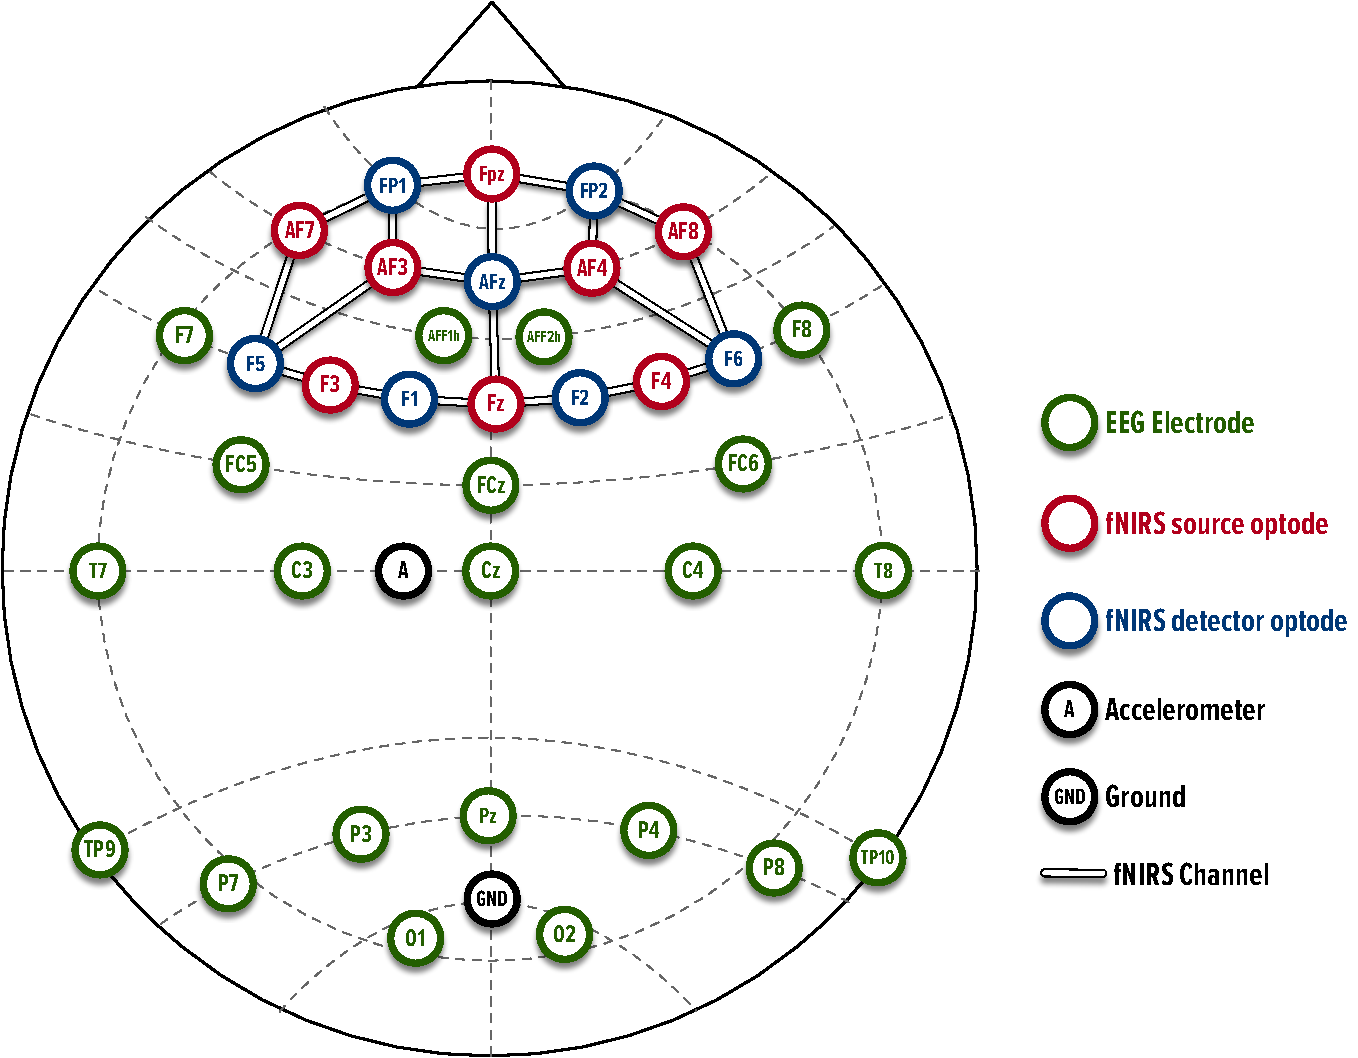
\includegraphics[width=\linewidth]{images/combined_montage.pdf}
  \centering
  \caption{%
      The montage we used for combined EEG/fNIRS data acquisition.  EEG
      electrodes were located in the anterior frontal (AFF1h, AFF2h), frontal
      (F7, F8), frontocentral (FC5, FCz, FC6), central (C3, Cz, C4),
      occipital (O1, O2), temporal (T7, T8) and parietal (P7, P3, Pz, P4, P8)
      regions.  fNIRS optodes were located in frontal (Fz, F1, F2, F3, F4,
      F5, F6), anterior frontal (AF3, AF4, AFz, AF7, AF8), frontal polar
      (FP1, FPz, FP2). The line is the channel formed when fNIRS source
      optode (red) and fNIRS detector (blue) optode are combined.
  }
  \label{fig:combined-montage}
\end{figure}

\begin{table}
\centering
\begin{tabularx}{\textwidth}{lX}
    \toprule
    EEG signal columns & Description (topological location of the subject's brain) \\
    \midrule
    \texttt{<subject>\_eeg\_AFF1h} & Left anterior frontal region \\
    \texttt{<subject>\_eeg\_F7} & Left frontal region  \\
    \texttt{<subject>\_eeg\_FC5} & Left fronto-central region  \\
    \texttt{<subject>\_eeg\_C3} & Left central region \\
    \texttt{<subject>\_eeg\_T7} & Left temporal region \\
    \texttt{<subject>\_eeg\_TP9} & Left temporal-parietal region \\
    \texttt{<subject>\_eeg\_Pz} & Central parietal region \\
    \texttt{<subject>\_eeg\_P3} & Left parietal region \\
    \texttt{<subject>\_eeg\_P7} & Left parietal region \\
    \texttt{<subject>\_eeg\_O1} & Left occipital region \\
    \texttt{<subject>\_eeg\_O2} & Right occipital region \\
    \texttt{<subject>\_eeg\_P8} & Right parietal region \\
    \texttt{<subject>\_eeg\_P4} & Right parietal region \\
    \texttt{<subject>\_eeg\_TP10} & Right temporal-parietal region \\
    \texttt{<subject>\_eeg\_Cz} & central region \\
    \texttt{<subject>\_eeg\_C4} & Right central region \\
    \texttt{<subject>\_eeg\_T8} & Right temporal region \\
    \texttt{<subject>\_eeg\_FC6} & Right fronto-central region \\
    \texttt{<subject>\_eeg\_FCz} & Central fronto-central region \\
    \texttt{<subject>\_eeg\_F8} & Right frontal region \\
    \texttt{<subject>\_eeg\_AFF2h} & Right anterior frontal region \\
    \texttt{<subject>\_eeg\_GSR} & Right hand \\
    \texttt{<subject>\_eeg\_EKG} & 4\textsuperscript{th} Intercostal space \\
    \bottomrule
\end{tabularx}
\caption{EEG signal descriptions, specifying the topological locations on the subject's brain. Each entry provides the label of the signal column corresponding to the EEG electrode location. For a visual representation of these electrode locations, refer to \autoref{fig:combined-montage}.
}
\label{tab:EEG_signals}
\end{table}

\begin{table}
  \footnotesize
  \centering
  \begin{tabularx}{\textwidth}{lX}
  \toprule
  fNIRS raw signal columns & Description (topological location of the subject's brain) \\
  \midrule
  \texttt{<subject>\_fnirs\_S1-D1\_760} & 'F3-F5': left frontal region \\
  \texttt{<subject>\_fnirs\_S1-D2\_760} & 'F3-F1': left frontal region  \\
  \texttt{<subject>\_fnirs\_S2-D1\_760} & 'Af7-F5': left anterior frontal region  \\
  \texttt{<subject>\_fnirs\_S2-D3\_760} & 'Af7-Fp1': left anterior frontal region  \\
  \texttt{<subject>\_fnirs\_S3-D1\_760} & 'Af3-F5': left anterior frontal region  \\
  \texttt{<subject>\_fnirs\_S3-D3\_760} & 'Af3-Fp1': left anterior frontal region  \\
  \texttt{<subject>\_fnirs\_S3-D4\_760} & 'Af3-Afz': left anterior frontal region  \\
  \texttt{<subject>\_fnirs\_S4-D2\_760} & 'Fz-F1': left frontal region  \\
  \texttt{<subject>\_fnirs\_S4-D4\_760} & 'Fz-Afz': central frontal region  \\
  \texttt{<subject>\_fnirs\_S4-D5\_760} & 'Fz-F2': right frontal region  \\
  \texttt{<subject>\_fnirs\_S5-D3\_760} & 'Fpz-Fp1': left frontal polar region  \\
  \texttt{<subject>\_fnirs\_S5-D4\_760} & 'Fpz-Afz': central frontal polar region  \\
  \texttt{<subject>\_fnirs\_S5-D6\_760} & 'Fpz-Fp2': right frontal polar region  \\
  \texttt{<subject>\_fnirs\_S6-D4\_760} & 'Af4-Afz': right anterior frontal region  \\
  \texttt{<subject>\_fnirs\_S6-D6\_760} & 'Af4-Fp2': right anterior frontal region  \\
  \texttt{<subject>\_fnirs\_S6-D7\_760} & 'Af4-F6': right anterior frontal region  \\
  \texttt{<subject>\_fnirs\_S7-D5\_760} & 'F4-F2': right frontal region  \\
  \texttt{<subject>\_fnirs\_S7-D7\_760} & 'F4-F6': right frontal region  \\
  \texttt{<subject>\_fnirs\_S8-D6\_760} & 'Af8-Fp2': right anterior frontal region  \\
  \texttt{<subject>\_fnirs\_S8-D7\_760} & 'Af8-F6': right anterior frontal region  \\
  \texttt{<subject>\_fnirs\_S1-D1\_850} & 'F3-F5': left frontal region  \\
  \texttt{<subject>\_fnirs\_S1-D2\_850} & 'F3-F1': left frontal region  \\
  \texttt{<subject>\_fnirs\_S2-D1\_850} & 'Af7-F5': left anterior frontal region  \\
  \texttt{<subject>\_fnirs\_S2-D3\_850} & 'Af7-Fp1': left anterior frontal region  \\
  \texttt{<subject>\_fnirs\_S3-D1\_850} & 'Af3-F5': left anterior frontal region  \\
  \texttt{<subject>\_fnirs\_S3-D3\_850} & 'Af3-Fp1': left anterior frontal region  \\
  \texttt{<subject>\_fnirs\_S3-D4\_850} & 'Af3-Afz': left anterior frontal region  \\
  \texttt{<subject>\_fnirs\_S4-D2\_850} & 'Fz-F1': left frontal region  \\
  \texttt{<subject>\_fnirs\_S4-D4\_850} & 'Fz-Afz': central frontal region  \\
  \texttt{<subject>\_fnirs\_S4-D5\_850} & 'Fz-F2': right frontal region  \\
  \texttt{<subject>\_fnirs\_S5-D3\_850} & 'Fpz-Fp1': left frontal polar region  \\
  \texttt{<subject>\_fnirs\_S5-D4\_850} & 'Fpz-Afz': central frontal polar region  \\
  \texttt{<subject>\_fnirs\_S5-D6\_850} & 'Fpz-Fp2': right frontal polar region  \\
  \texttt{<subject>\_fnirs\_S6-D4\_850} & 'Af4-Afz': right anterior frontal region  \\
  \texttt{<subject>\_fnirs\_S6-D6\_850} & 'Af4-Fp2': right anterior frontal region  \\
  \texttt{<subject>\_fnirs\_S6-D7\_850} & 'Af4-F6': right anterior frontal region  \\
  \texttt{<subject>\_fnirs\_S7-D5\_850} & 'F4-F2': right frontal region  \\
  \texttt{<subject>\_fnirs\_S7-D7\_850} & 'F4-F6': right frontal region  \\
  \texttt{<subject>\_fnirs\_S8-D6\_850} & 'Af8-Fp2': right anterior frontal region  \\
  \texttt{<subject>\_fnirs\_S8-D7\_850} & 'Af8-F6': right anterior frontal region  \\
  \bottomrule
  \end{tabularx}
  \caption{Table of fNIRS raw signal descriptions, mapping the source (S) to the detector (D) for various topological locations on the subject's brain. These signals where recorded using the Aurora fNIRS software. Each channel is recorded using light wavelengths of 760nm and 850nm. For a visual representation of these electrode locations, refer to \autoref{fig:combined-montage}.}
  \label{tab:fNIRS_raw_signals}
  \end{table}

  \begin{table}
      \footnotesize
    \centering
    \begin{tabularx}{\textwidth}{lX}
    \toprule
    fNIRS raw signal columns & Description (topological location of the subject's brain) \\
    \midrule
    \texttt{<subject>\_fnirs\_S1-D1\_HbO} & 'F3-F5': left frontal region \\
    \texttt{<subject>\_fnirs\_S1-D2\_HbO} & 'F3-F1': left frontal region  \\
    \texttt{<subject>\_fnirs\_S2-D1\_HbO} & 'Af7-F5': left anterior frontal region  \\
    \texttt{<subject>\_fnirs\_S2-D3\_HbO} & 'Af7-Fp1': left anterior frontal region  \\
    \texttt{<subject>\_fnirs\_S3-D1\_HbO} & 'Af3-F5': left anterior frontal region  \\
    \texttt{<subject>\_fnirs\_S3-D3\_HbO} & 'Af3-Fp1': left anterior frontal region  \\
    \texttt{<subject>\_fnirs\_S3-D4\_HbO} & 'Af3-Afz': left anterior frontal region  \\
    \texttt{<subject>\_fnirs\_S4-D2\_HbO} & 'Fz-F1': left frontal region  \\
    \texttt{<subject>\_fnirs\_S4-D4\_HbO} & 'Fz-Afz': central frontal region  \\
    \texttt{<subject>\_fnirs\_S4-D5\_HbO} & 'Fz-F2': right frontal region  \\
    \texttt{<subject>\_fnirs\_S5-D3\_HbO} & 'Fpz-Fp1': left frontal polar region  \\
    \texttt{<subject>\_fnirs\_S5-D4\_HbO} & 'Fpz-Afz': central frontal polar region  \\
    \texttt{<subject>\_fnirs\_S5-D6\_HbO} & 'Fpz-Fp2': right frontal polar region  \\
    \texttt{<subject>\_fnirs\_S6-D4\_HbO} & 'Af4-Afz': right anterior frontal region  \\
    \texttt{<subject>\_fnirs\_S6-D6\_HbO} & 'Af4-Fp2': right anterior frontal region  \\
    \texttt{<subject>\_fnirs\_S6-D7\_HbO} & 'Af4-F6': right anterior frontal region  \\
    \texttt{<subject>\_fnirs\_S7-D5\_HbO} & 'F4-F2': right frontal region  \\
    \texttt{<subject>\_fnirs\_S7-D7\_HbO} & 'F4-F6': right frontal region  \\
    \texttt{<subject>\_fnirs\_S8-D6\_HbO} & 'Af8-Fp2': right anterior frontal region  \\
    \texttt{<subject>\_fnirs\_S8-D7\_HbO} & 'Af8-F6': right anterior frontal region  \\
    \texttt{<subject>\_fnirs\_S1-D1\_HbR} & 'F3-F5': left frontal region  \\
    \texttt{<subject>\_fnirs\_S1-D2\_HbR} & 'F3-F1': left frontal region  \\
    \texttt{<subject>\_fnirs\_S2-D1\_HbR} & 'Af7-F5': left anterior frontal region  \\
    \texttt{<subject>\_fnirs\_S2-D3\_HbR} & 'Af7-Fp1': left anterior frontal region  \\
    \texttt{<subject>\_fnirs\_S3-D1\_HbR} & 'Af3-F5': left anterior frontal region  \\
    \texttt{<subject>\_fnirs\_S3-D3\_HbR} & 'Af3-Fp1': left anterior frontal region  \\
    \texttt{<subject>\_fnirs\_S3-D4\_HbR} & 'Af3-Afz': left anterior frontal region  \\
    \texttt{<subject>\_fnirs\_S4-D2\_HbR} & 'Fz-F1': left frontal region  \\
    \texttt{<subject>\_fnirs\_S4-D4\_HbR} & 'Fz-Afz': central frontal region  \\
    \texttt{<subject>\_fnirs\_S4-D5\_HbR} & 'Fz-F2': right frontal region  \\
    \texttt{<subject>\_fnirs\_S5-D3\_HbR} & 'Fpz-Fp1': left frontal polar region  \\
    \texttt{<subject>\_fnirs\_S5-D4\_HbR} & 'Fpz-Afz': central frontal polar region  \\
    \texttt{<subject>\_fnirs\_S5-D6\_HbR} & 'Fpz-Fp2': right frontal polar region  \\
    \texttt{<subject>\_fnirs\_S6-D4\_HbR} & 'Af4-Afz': right anterior frontal region  \\
    \texttt{<subject>\_fnirs\_S6-D6\_HbR} & 'Af4-Fp2': right anterior frontal region  \\
    \texttt{<subject>\_fnirs\_S6-D7\_HbR} & 'Af4-F6': right anterior frontal region  \\
    \texttt{<subject>\_fnirs\_S7-D5\_HbR} & 'F4-F2': right frontal region  \\
    \texttt{<subject>\_fnirs\_S7-D7\_HbR} & 'F4-F6': right frontal region  \\
    \texttt{<subject>\_fnirs\_S8-D6\_HbR} & 'Af8-Fp2': right anterior frontal region  \\
    \texttt{<subject>\_fnirs\_S8-D7\_HbR} & 'Af8-F6': right anterior frontal region  \\
    \bottomrule
    \end{tabularx}
    \caption{%
        fNIRS raw signal descriptions, mapping the source (S) to the detector
        (D) for various topological locations on the subject's brain. HbO, or
        oxyhemoglobin, and HbR, or deoxyhemoglobin, are the two types of
        hemoglobin measured. For a visual representation of these electrode
        locations, refer to \autoref{fig:combined-montage}.
    }
    \label{tab:fNIRS_signals}
    \end{table}

\section{Derived data}

\subsection{Synchronization of EEG, EKG, GSR, and fNIRS Signals}

In multimodal neuroimaging studies, synchronizing signals from multiple modalities is a crucial step to conducting comprehensive studies on all these modalities together. The discrepancy between EEG and fNIRS signals' time series is an issue that researchers encounter frequently due to the limitations of recording hardware or the necessity to remove invalid signals. Additionally, these two modalities have distinct recording rates, further complicating their alignment. To facilitate comprehensive evaluation of EEG and fNIRS signals, it is essential to synchronize these two signals.

The synchronization process is a two-step approach involving the noise artifacts removal from the signals, followed by resampling and synchronization of the interpolated signals at the desired sampling rate.

\subsubsection{Removing Noise in EEG Signals with Notch Filter}

EEG signals often exhibit susceptibility to artifacts, an interference that can be attributed to several sources. For instance, physiological factors such as eye movements or blinks can induce such artifacts \cite{10.3389/fnhum.2012.00278}, as can environmental elements like fluorescent lighting or grounding complications \cite{Kaya21}.

Upon thorough examination and visualization of the raw EEG data, we identified a consistent 60 Hz electrical disturbance within the signal, along with corresponding harmonics. An anomalous peak was also noted around the 5 Hz mark, potentially attributable to a grounding irregularity or an other environmental factors.

With the aid of MNE-Python \cite{GramfortEtAl2013a}, we efficiently mitigated these intrusive noises by deploying a notch filter. The filter was configured with a frequency of 60 Hz, a transition bandwidth of 9 Hz, and notch widths of 2 Hz.

\subsubsection{Mitigating Artifacts in fNIRS Signals Utilizing Bandpass Filter}

fNIRS signals are often susceptible to motion artifacts (MA) stemming from physiological activities, including cardiac and respiratory disturbances. These artifacts become particularly noticeable in the measurement of oxyhemoglobin (HbO) and deoxyhemoglobin (HbR) concentrations within the signal channels.

To address these challenges, we employed a bandpass filter as an effective noise reduction strategy. The filter was calibrated in line with the recommendations provided by \cite{Koenraadt2014}. With a low cutoff bandwidth of 0.01 Hz and a high cutoff bandwidth of 0.2 Hz for the 4th order Butterworth method, the filter was tailored to selectively allow signal components within this frequency range while attenuating components outside the range.

\subsubsection{Pre-processing EKG and GSR Signals}

To remove noise and improve peak-detection accuracy for EKG signals, we employed a finite impulse response (FIR) filter with 0.67 Hz low cutoff frequency, 45 Hz high cutoff frequency, and order of $1.5 \times \text{sampling rate}$ (where sampling rate is 500 Hz) implemented by NeuroKit2 \cite{Makowski2021neurokit}.

We removed noise and smoothed the GSR signals using a low-pass filter with a 3 Hz cutoff frequency and a $4^\text{th}$ order Butterworth filter, both implemented by Neurokit2.

\subsubsection{Synchronization of EEG, EKG, GSR, and fNIRS Signals}

After the EEG, EKG, GSR, and fNIRS signals are pre-processed to remove noise, the signals are resampled to a common sampling rate using the FFT-based resampling method \texttt{mne.filter.resample} available in the Python MNE library \cite{GramfortEtAl2013a}. To synchronize the signals, we generate a time series matching the common sampling rate of the resampled signals, with the first timestamp rounded to the nearest second. Then, the signals are interpolated to this generated time series via linear interpolation.

\subsection{Synchronizing Task Data with EEG and fNIRS Resampled Signals}

Understanding the relationship between participants' behaviors, environmental stimuli, and neuroimaging data requires a precise synchronization of task data with the corresponding EEG and fNIRS signals. By aligning these data streams, we can examine the influence of environmental stimuli on the participants' neuroimaging signals, which in turn, impact their behavior and task performance.

The process of integrating EEG and fNIRS signals with task data starts with grouping of signals by the tasks during which they were recorded, followed by the synchronization of the task data to the corresponding EEG and fNIRS signals.

\subsubsection{Grouping EEG, EKG, GSR, and fNIRS Signals by Task}

The preliminary step in our approach to synchronizing EEG, EKG, GSR, and fNIRS signals with the task data involves the grouping of the signals by the tasks during which the signals were recorded. The task data can be categorized into two distinct types: status-based and event-based data.

\paragraph{Status-based task data} This type of task data represent the current state of the task, such as task score. For each task, the grouping process of these data begins by including the signals recorded immediately before the task initiation and immediately following task completion. This ensures no data is overlooked at the boundaries of the task. Subsequently, all signals recorded between these two points are included, forming a complete set of signals associated with the task.

\paragraph{Event-based task data} This type of task data, on the other hand, correspond to specific events that occur during the task, such as affective task arousal or the submission of a valence score. For each task, we determine the EEG, EKG, GSR, and fNIRS entry associated with the first event and the last event. These signal entries, as well as all entries recorded between these points, are included into the data set related to the task.

\subsubsection{Synchronizing Task Data with EEG, EKG, GSR, and fNIRS Signals}

Having grouped the EEG, EKG, GSR, and fNIRS signals according to task type, we then proceed to synchronize these signal entries with their respective task data.

\paragraph{Status-based task data} The synchronization is accomplished by assigning the status data recorded closest in time to each EEG, EKG, GSR, and fNIRS signal entry. This method ensures that each EEG, EKG, GSR, and fNIRS entry is paired with the most representative status data.

\paragraph{Event-based task data} We assign each event data to the EEG, EKG, GSR, and fNIRS signal entry recorded at the time closest to the occurrence of the event. Those EEG, EKG, GSR, and fNIRS signal entries without a corresponding event data are left unassigned, signifying that no specific event occurred during these recordings.